%% ===============================================================================================
%% @author Leonardo Florez-Valencia (florez-l@javeriana.edu.co)
%% ===============================================================================================

\documentclass[letter]{article}

\usepackage[spanish]{babel}
\usepackage[margin=1in]{geometry}
\usepackage{amsmath}
\usepackage{amsthm}
\usepackage{amssymb}
\usepackage[utf8]{inputenc}
\usepackage{graphicx, color}
\usepackage{algorithm}
\usepackage{algpseudocode}
\usepackage{mathrsfs}

% Some definitions
\floatname{algorithm}{Algoritmo}

% Author info
\title{Taller dividir y vencer}
\author{Jose Fernando Zuluaga, Nicolas Daniel Vargas}
\date{
	$^1$Departamento de Ingeniería de Sistemas, Pontificia Universidad Javeriana\\Bogotá,  Colombia \\
	\texttt{\{zuluaga\_jose@javeriana.edu.co}\\~\\
	\today
}

\begin{document}
\maketitle
	
\begin{abstract}
En este documento se presenta la documentación correspondiente al taller 2 de análisis de algoritmos, donde se basa el desarrollo y descripción de los algoritmos planteados como solución
\textbf{Palabras clave:} iterativo, algoritmo, formalización, experimentación, complejidad, dividir y vencer.
\end{abstract}

\tableofcontents
	
\section{Introducción} \label{intro}
Los numeros naturales tienen su representación binaria, en ceros y unos, esta representación se puede ver como una secuencia de estos numeros, donde su ubicación e índice es relevante para su estructura. Como proposito del taller es trabajar con esta relación de numeros naturales y su representación binaria para escribir los algoritmos que lleguen a al resultado requerido.

\section{Formalización del problema} \label{formalizacion}
El problema recibe incialmente un numero $n\in \mathbb{N}$, se busca y opera su representación binaria. Esto con el fin, de hallar su representación binaria inversa, como requisito para el desarrollo del taller se pide dos algoritmos diferentes, el primero iterativo, y un segundo recursivo utilizando la tecnica dividir y vencer.

\subsection{Definición del problema del ``numero binario inverso''} \label{problema}
Así, el problema de la representación binaria inveresa se define a partir de:
  \begin{enumerate}
    \item un numero $n$ tal que $n\in \mathbb{N}$ y donde $-2,147,483,647<n<2,147,483,647$, restricción para el usuario
    \item una secuencia de numeros $S$ que contiene la representación binaria de $n$
  \end{enumerate}
producir un nuevo numero $n'$ cuyo valor es la representación decimal de la secuencia inversa de $S$
\begin{itemize}
    \item Entradas:
    \begin{itemize}
        \item $n\in \mathbb{N}$
    \end{itemize}
    \item Salidas:
    \begin{itemize}
        \item $n'\in \mathbb{N}$
    \end{itemize}
\end{itemize}

\section{Algoritmos de solución} \label{algoritmos}
\subsection{Iterativa}
El algoritmo iterativo maneja un arreglo de numeros enteros, en el cual almacena la representación binaria inversa del numero recibido. Se manejan dos ciclos, el primer ciclo tiene como función calcular la representación binaria inversa del numero, en este se guarda en la posicion i del arreglo mecionado el reciduo de la de division $n/2$ , acto seguido se divide el numero $n$ entre dos, esto se repetira mientras $n \neq 0$. El segundo ciclo se utiliza para la transformación de la representación binaria inversa obtenida a un numero decimal y se hara uso de dos variables extra que son num,el cual es el numero decimal deseado($n'$) y exp que sera el exponente de la ubicacion,en este ciclo se recorre el arreglo $S'$ verificando cuales valores son 1, si lo es entonces se eleva 2 a la exp y eso se le suma a la variable num. Finalmente se muestra en pantalla el numero obtenido  $n'$.



\begin{algorithm}[!htb]
\caption{Version Iterativa}
\begin{algorithmic}[1]
\Require $S=\left< S_i = 1 | 0 \right>$, $n \in \mathbb{N}$
\Ensure $n$ será convertido a expresión binaria, $S$ contendrá la expresión binaria de $n$
\Procedure{ToBin}{$n, S$}
  \For{$i \leftarrow 0~\mathbf{to}~n<>0$}
    \State$s_i \leftarrow n MOD~2$
    \State$n \leftarrow n/2$
  \EndFor
\EndProcedure\\

\Procedure{ToDec}{$n, e, S$}
  \For{$i \leftarrow |S|-1~\mathbf{to}~i=0$}
    \If{$S_i = 1$}
      \State$n \leftarrow n+ 2^e$
      \State $e++$
    \EndIf
    \State$i--$
  \EndFor
\EndProcedure
\end{algorithmic}
\end{algorithm}

\subsubsection{Análisis de complejidad} \label{algoritmos:mejorado:complejidad}

Por inspección de código: hay dos ciclos {\it para-todo} no anidados que, en el peor de los casos, recorren todo la secuencia de datos; entonces, este algoritmo es $O(|S|)$.



\subsection{Recursivo usando dividir y vencer} \label{algoritmos:recursivo}
Para iniciar este algoritmo convierte el numero decimal ingresado $n$ en binario haciendo uso de una funcion recursiva que guarda en una lista $S$ la forma binaria inversa del numero $n$, esto se guarda de forma inversa ya que asi es la forma en la que se calcula el numero binario de $n$ pero ya que lo que se nos pide es la representació binaria de este entonce se implementa un funcion que recibira la posicion del inicio del arreglo $ini$ y la posicion final del arreglo $tam$, el objetivo de esta funcion es comparar la posicion inicial y final de la lista, si estas dos son iguales entonces se tomara el caso base en donde se guarda el valor en una lista auxiliar $S'$ que llamaremos numeros nuevos, de lo contrario se parte la lista $S$ en dos partes con ayuda de un pivote $q$, luego de esto la funcion se llama a si misma dos veces, una enviando solo la mitad derecha de la lista $S$ y la otra la mitad izquierda, es decir, en el caso del lado derecho el inicio $ini$ de la lista que se envia sera $q+1$ y la posicion final $tam$ sera el mismo $tam$ original, mientras que el lado izquierdo comprendera desde $ini$ hasta $q$, siempre se envia primero la parte derecha de la lista para asi guardar la lista desde el ultimo elemento hasta el primero.
Finalmente se nos pide convertir el numero binario inverso , que se encuentra dentro de la lista $S'$, en su representación decimal, para esto haremos uso de la función ''desbinarización" la cual recibe como parametros el inicio ($ini$) y final ($tam$) de la lista, un entero que llamaremos ''respuesta'' y un exponente que llamaremos ''exp'',estos ultimos dos empiezan en cero y se pasan como parametros para poder manjarlo dentro de la funcion la cual al igual que la funcion anterior parte la lista en dos con ayuda de un pivote $q$, no obstante, en el caso base despues de comparar el $ini$ y $tam$ reviza si el valor que se tiene llamemoslo $v$ es igual a $1$, si es asi entonces entonces a ''respuesta'' se le suma  $2^{exp}$ y se aumenta $exp$ en $1$, si en caso contrario $v$ no es $1$ entonces solo se aumenta $exp$ en $1$. Al igual que la función anteriormente descrita, ''desbinarización'' reviza primero la parte derecha del arreglo que recibe 

\begin{algorithm}[!htb]
\caption{Versión Dividir y vencer}
\begin{algorithmic}[1]
\Require $n \in \mathbb{N}$
\Ensure $n$ será tranformado a su expresión binaria, $S$ contendra la expresión binaria de $n$, $Z$ contendrá la expresión binaria inversa de $n$ 
\Procedure{ToBin}{$n$}
  \If{$n <> 0$}
    \State \Call {S.push\_back}{$n~MOD~2$}
    \State \Call {ToBin}{$n/2$}
  \EndIf
\EndProcedure\\
\end{algorithmic}


\begin{algorithmic}[1]
\Procedure{Reverse}{$i, f$}
  \If{$i=f$}
  \State $q \leftarrow S_i$
  \State \Call{Z.push\_back}{$q$}
  \EndIf
  \If{$i <> f$}
  \State $p \leftarrow (i+f)/2$
  \State \Call{Reverse}{$p+1, f$}
  \State \Call{Reverse}{$i, p$}
  \EndIf
\EndProcedure\\
\end{algorithmic}

\begin{algorithmic}[1]
\Procedure{ToDec}{$n, e, i, f$}
\If{$i=f$}
    \If{$Z_f~=~1$}
        \State $n\leftarrow n+2^e$
    \EndIf
    \State $e\leftarrow e+1$
    \If{$Z_f <> 1$}
        \State $q \leftarrow (f+i)/2$
        \State \Call{ToDec}{$n, e, q+1, f$}
        \State \Call{ToDec}{$n, e, i, q$}
    \EndIf
\EndIf
\EndProcedure
\end{algorithmic}

\end{algorithm}

\subsubsection{Análisis de complejidad} \label{algoritmos:recursivo:complejidad}

Como podemos ver en el codigo de la funcion reverse se hacen dos llamados recursivos y siempre se parten los datos en dos partes, las partes del algoritmo que no son recursivas tampoco son iterativos, por ende, si hacemos uso de la formula del teorema maestro obtenemos una complejidad de

\[T(n)= 2T(n/2)+O(1) \]

\[1= n^{log_2(2-E)} \rightarrow E=1\]
\[1= n^{log_2(2)}log_2^kn \rightarrow \]
\[1= n^{log_2(2+E)} \rightarrow E=-1\]

Como podemos ver el caso mas optimo es el primero donde $E = 1$ por ende podemos concluir que este caso tiene una complejidad

\[\theta(n^{log_22})\]
\[\theta(n)\]

\section{Análisis Experimental}
Para la parte experimental de nuestro taller, se realizo una tabla con ciertos datos a tener en escenarios de prueba como lo es:
\begin{itemize}
    \item \textbf{Numero ingresado}: Representa el numero ingresado por el usuario
    \item\textbf{Inverso Deseado}: Representa el numero teórico, el numero que se debería de recibir como resultado
    \item\textbf{Inverso obtenido: }Representa el numero experimental, el numero recibido como resultado por el algoritmo
    \item\textbf{Tiempo: }Representa el tiempo que tardo el algortimo durante su ejecución
    \item\textbf{Tendencia: }Representa la tendencia del algortimo durante su ejecución\\
\end{itemize}

Como observamos de los resultados, la tendencia es constante su cambio es poco notable, a diferencia del tiempo, que es tomado en microsegundos, es realmente muy poco en tiempo de ejecución, teniendo en cuenta las propiedades del entorno de ejecución. Concluimos que la complejidad efectivamente, como fue mencionado anteriormente, es \[\theta(n)\]
\begin{figure}[h]
\centerline{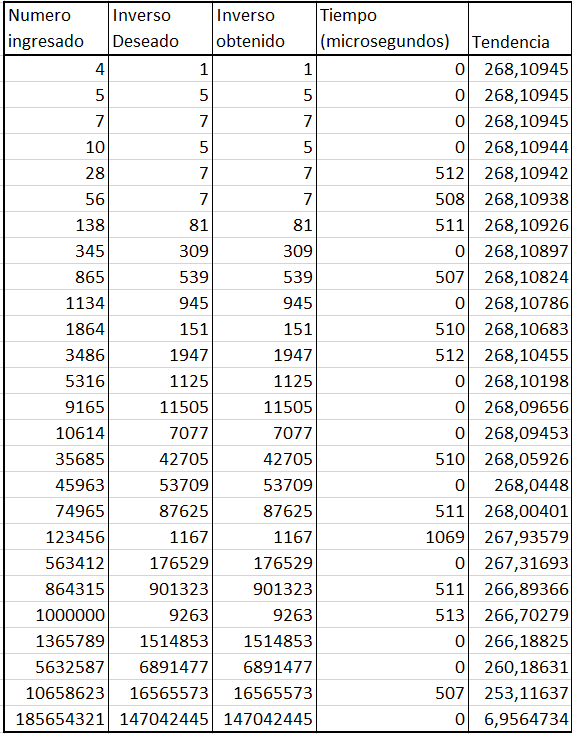
\includegraphics[scale=1]{images/Tabla de datos.PNG}}
\caption{Tabla de datos y resultados.}
\label{table}
\end{figure}


\begin{figure}[h]
\centerline{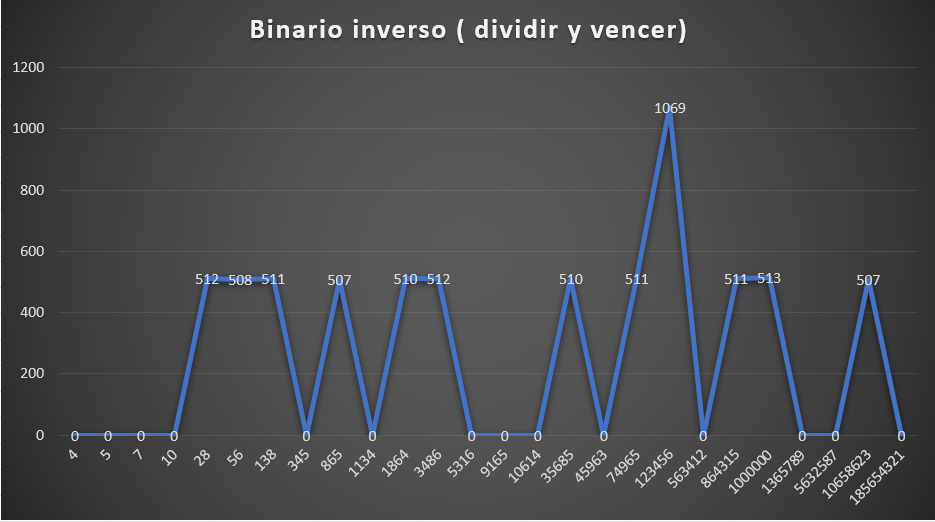
\includegraphics[scale=1]{images/Grafica.PNG}}
\caption{Grafica resultado.}
\label{graph}
\end{figure}

\end{document}

%% eof - sorting.tex
